\chapter{Konzept}
\label{chap:concept}

Dieses Kapitel widmet sich dem Konzept der vorliegenden Arbeit, wie
die Anforderungen, die in Abschnitt~\ref{sec:aim}
angedeutet wurden genauer aussehen und gelöst werden können.\\
Dazu wird zunächst der grobe Aufbau der Arbeit beschrieben und
anschließend die einzelnen Funktionen.

\section{Architektur}

Architektonisch soll diese Arbeit, im Folgenden "`YAVA"' (Yet Another Vegan App)
genannt, so aussehen, wie in Abbildung~\ref{img:concept} schematisch dargestellt ist.

\begin{figure}[ht]
	\centering
	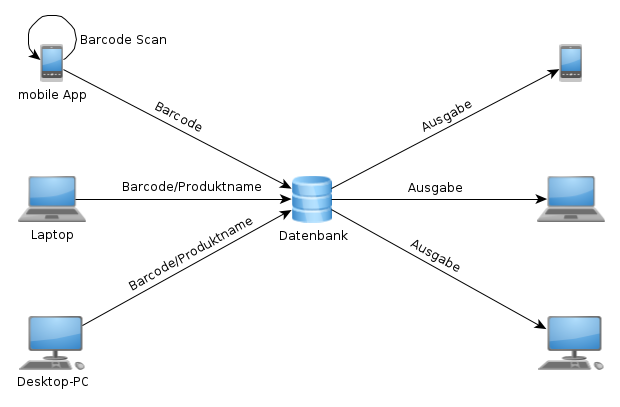
\includegraphics[scale=0.7]{misc/concept.png}
	\caption{Grober schematischer Aufbau von \name}
	\label{img:concept}
\end{figure}

Zu sehen sind drei Systeme: die mobile Anwendung, die Webanwendung
auf einem Laptop und die Webanwendung auf einem Desktop-PC.
Die drei unterschiedlichen Systeme sollen die Plattformunabhängigkeit symbolisieren.
Alle drei Systeme können Eingaben an die Datenbank schicken.
Dabei kann mit der mobilen App mit
Hilfe eines Barcodescanners ein Barcode gescannt werden, der als
Sucheingabe benutzt wird, die jeweiligen Webanwendungen bieten die Möglichkeit
zusätzlich zu einer manuell eingegebenen
GTIN auch nach einem Produktnamen zu suchen.
Die jeweilige Eingabe wird an die Datenbank gesendet, die die
entsprechenden Produkte bzw. Einträge finden soll und im Erfolgsfall ausgibt.
Die Darstellung erfolgt jeweils wieder auf dem Endgerät.\\
Die im Ziel definierte Anforderung, eine plattformunabhängige Produktdatenbank
aufzubauen, ist hier zu erkennen. Die weiteren Anforderungen und die einzelnen Komponenten dazu
werden im Folgenden beschrieben.

\subsection*{Datenbank}
\label{sec:concept:db}

Die Datenbank enthält alle Daten und bildet somit den Kern dieser
Arbeit. Mit ihr können die Webanwendung und die Apps kommunizieren um
Daten hinzuzufügen, zu ändern, zu löschen oder anzuzeigen.
Die Datenbank ist von außerhalb nicht zugänglich und kann nur über die
Schnittstellen Webanwendung bzw. mobile App benutzt werden.
Um die freie Nutzung der Daten zu gewährleisten gibt es jedoch einen
täglichen Speicherauszug dieser Datenbank (ohne die sensitiven
Informationen der Nutzer*innen), die auf einer Website angezeigt
werden und heruntergeladen werden können.\\
Der Aufbau der Datenbank wird in Abschnitt~\ref{sec:implementation:db}
beschrieben.

\subsection*{Mobile App}
\label{sec:concept:app}

Die mobile Anwendung, die "`YAMVA"' (Yet Another Mobile Vegan App) genannt wurde,
ist hauptsächlich dafür gedacht, die Suche nach einem
Produkt zu erleichtern, indem einfach der Barcode-Scanner benutzt
werden kann. Nach dem Scan eines Barcodes wird -- eine bestehende
Internetverbindung vorausgesetzt -- in der Datenbank (vgl. Abschnitt~\ref{sec:concept:db})
danach gesucht und das
Ergebnis angezeigt.
Befindet sich das gescannte Produkt nicht in der Datenbank, kann durch
einen Link von der mobilen App zur Webanwendung
gewechselt werden, um dort das Produkt eintragen zu können. Ansonsten kann ebenfalls
über einen Link zur Webanwendung gewechselt werden, um mehr Informationen über das gescannte Produkt zu erhalten.
Die Webanwendung adaptiert sich dank
"`responsive Webdesign"', also einem Webdesign, was sich an die jeweiligen 
Endgeräte anpasst, auch an das mobile Endgerät.

\subsection*{Webanwendung}
\label{sec:concept:webapp}

Die Webanwendung ist das Frontend der Datenbank.
Sie besteht aus einer Bedienoberfläche und kann somit zur Verwaltung
von allen Daten gebraucht werden. Es können sich hier Nutzer*innen
anmelden, um Daten neu hinzuzufügen, zu ändern oder zu löschen und
alle Daten können damit dargestellt werden.
Die Webanwendung kommuniziert im Hintergrund ständig mit der Datenbank
um diese Daten zu verwalten
und kann durch das responsive Webdesign
auf allen Geräten angezeigt werden.\\
Der Funktionsumfang wird in Abschnitt~\ref{sec:concept:functions} beschrieben.

\section{Integration in das \acl{IRL}}
\label{sec:concept:irl}

Das \acf{IRL} ist ein "`Living Lab"', ein 
anwendungsnahes und Nutzer*innenzentriertes Forschungslabor des Deutschen 
Forschungszentrums für Künstliche Intelligenz (DFKI), das in der Zentrale der 
Globus SB-Warenhaus Holding in St. Wendel eingerichtet ist \citeweb{irl, dfki, 
globus, irl:partner}, \cite{sskk09}.
In diesem Living Lab gibt es diverse Demonstratoren, die verschiedene Prozesse 
beim Einkaufen erleichtern. Z.\,B. ist dort der "`Artikelfinder"', ein 
Terminal, an dem nach Produkten gesucht werden kann und im Erfolgsfall der 
Standort angezeigt wird, integriert \citeweb{irl:artikelfinder}.
Da die vorliegende Arbeit auch in einem realen Warenhaus als Assistenzsystem 
eingesetzt werden kann, soll auch \name im \ac{IRL} als Demonstrator 
integriert werden.\\
Da die Daten, die innerhalb des \ac{IRL} verwendet werden, aus
rechtlichen Gründen nicht
veröffentlicht werden dürfen, wird \name mit den einzelnen Komponenten
(Webanwendung, Datenbank und mobiler App)
als eigener Dienst im \ac{IRL} neu aufgebaut.

\section{Layout}
\label{sec:concept:layout}

Im Folgenden wird kurz beschrieben, wie das Layout von \name aussehen soll.
Die Anzeigen, die auf den einzelnen Seiten dargestellt werden, werden zum Teil 
in den nachfolgenden Abschnitten erläutert.

\subsection{Startseite}
\label{sec:concept:dashboard}

Auf der Startseite
sollen sich neben einer Begrüßung eine Möglichkeit zur
Registrierung bzw. Anmeldung befinden und die fünf neuesten Produkte, die
eingetragen wurden.
Sobald sich ein*e Nutzer*in angemeldet hat, sollen sich zusätzlich
zu den fünf neuesten Produkten fünf Produkte befinden, die noch nicht 
vollständig eingetragen wurden
(vgl. Abschnitt~\ref{sec:concept:gamification}), um so direkt die Aufmerksamkeit
auf diese Produkte zu lenken.\\
Die Navigation soll sich im oberen Bereich befinden und Links zur Startseite selbst, den
Produkten, Zutaten, Hersteller*innen, Nutzer*innen und ein Dropdown-Menü beinhalten.
Dieses Menü ist mit dem
Nutzer*in-Namen und der aktuellen Punktanzahl in Klammern beschriftet
und enthält Links zu der
Übersichtsseite von einem*einer Nutzer*in, den Nutzer*in-Einstellungen
und einen Link zum Abmelden.\\
Die Fußzeile dagegen soll Links zur Website des Autors, der
Sitemap, den FAQ, zum Kontakt, zu News sowie zu den Terms of
Service, die die Richtlinien von \name definieren, enthalten.

\subsection{Produktanzeige}
\label{sec:concept:view}

In der Ansicht eines vollständig eingetragenen Produktes
(siehe Abschnitt~\ref{sec:concept:product}) sind folgende Informationen
aufgelistet bzw. zu sehen:

\begin{itemize}
		\item Name des Produktes
		\item Verpackungsgröße, z.\,B. "`500ml"'
		\item Marke mit dem*r zugehörigen Hersteller*in
		\item Barcode bzw. \ac{GTIN} % optional mit Bild
		\item Bild
		\item Produktbeschreibung
		\item Veganität, siehe dazu \ref{sec:concept:veganity}
		\item Zutatenliste
		\item Allergene
		\item Spuren von Allergenen
		\item geparste Zutaten anhand der Zutatenliste, siehe dazu
				\ref{sec:concept:ingredients}
		\item Kategorie, z.\,B. "`Milch und Alternativen"'
		\item Nährwertangaben mit Lebensmittelampel und \ac{GDA} % Bild, 
Link?
		\item Verpackungsmaterial, z.\,B. "`Grünes Glas"'
		\item Herkunftsland
		\item Siegel wie das V-Label \citeweb{vlabel}
		\item Merkmale wie z.\,B. "`glutenfrei"'
		\item Vollständigkeitsanzeige in Prozent -- so kann erkannt
				werden, was noch fehlt, siehe 
\ref{sec:concept:gamification} % auf der Startseite anzeigen
		\item Quelle, z.\,B. Link zu schon vorhandener Produktanfrage
				auf einem Blog
		\item Produktanfragen, siehe \ref{sec:concept:inquiries}
		\item Kommentare, siehe \ref{sec:concept:comments}
		\item Zeitangaben wie Erstellung und letzte Änderung mit
				Nutzer*inangaben
\end{itemize}

Angaben wie Veganität, Zutaten, Lebensmittelampel,
Vollständigkeitsanzeige, Produktanfragen, Kommentare sowie Zeit- und
Nutzer*inangaben werden automatisch generiert bzw. von anderen
Nutzer*innen erstellt und können nicht
oder nur eingeschränkt verändert werden.

\section{Funktionsumfang}
\label{sec:concept:functions}

Im Folgenden wird näher beschrieben, was mit Hilfe der Webanwendung
alles möglich ist und wie die Anforderungen (vgl.
Abschnitt~\ref{sec:aim}) damit erfüllt werden können.

\subsection{Produktsuche}
\label{sec:concept:search}

Eine zentrale Funktion einer Webanwendung ist die Suche, mit der nach
bestimmten Inhalten gesucht und somit eine einfachere Seitennavigation
ermöglicht werden kann.\\
Innerhalb von \name ist eine Suche nach dem Barcode bzw. der \ac{GTIN}
sowie nach dem Produktnamen möglich.
Wenn ein einziges Ergebnis gefunden wurde, wird es direkt angezeigt,
wurden mehrere gefunden, werden diese aufgelistet und wenn kein
Produkt gefunden wurde, kann ein neues Produkt
angelegt werden.
Dieses enthält -- abhängig von der Sucheingabe --
entweder den Barcode oder den Produktnamen schon im Formular, in dem
das Produkt eingetragen werden kann.

\subsection{Registrierung \& Anmeldung}
\label{sec:concept:users}

Um Produkte oder andere Daten verwalten zu können, muss ein*e
Benutzer*in sich erst registrieren, um u.\,a. einer ersten Hürde der
Missbrauchsgefahr aus dem Weg zu gehen.
Ohne Registrierung bzw. Anmeldung können Daten nur eingesehen, aber
nicht verändert werden.\\
Die Registrierung geschieht über einen externen Dienst, von dem Daten wie Name, 
E-Mail\-adresse und Spitzname übernommen werden.
Nach der Registrierung soll eine E-Mail an die angegebene E-Mailadresse 
versendet werden um den*die Nutzer*in zu begrüßen und gleichzeitig diese Adresse 
auf Existenz und Gültigkeit zu validieren und anschließend eine Übersichtsseite 
angezeigt werden.
Diese beinhaltet ein Avatar (Bild von einem*einer Nutzer*in) zur leichteren 
Identifizierung,
welches mit Hilfe von "`Gravatar"', einem Webservice für global
eindeutige Avatare \citeweb{gravatar}, generiert wird. Dazu werden Punkte
(vgl. \ref{sec:concept:gamification}), ein Spitzname, die angelegten Produkten 
und 
Produktanfragen
und persönliche Informationen wie Name, E-Mailadresse und Rechte
(vgl. \ref{sec:concept:gamification}) angezeigt.
Ebenso gibt es hier die Möglichkeit den Account zu deaktivieren, wobei
alle privaten Daten anonymisiert werden und nicht wiederhergestellt
werden können. Außerdem kann hier der volle Name anonymisiert werden, sodass er 
innerhalb einer Produktanfrage als "`XYZ"' auf einer Produktübersicht angezeigt 
wird (vgl. \ref{sec:concept:inquiries}) und es können dort Daten wie Name, 
E-Mailadresse und Spitzname geändert werden.\\
Eine Anmeldung erfolgt wieder über einen Klick auf den entsprechenden Button
eines externen Dienstes, wobei nicht erneut der Zugriff auf
persönliche Daten erlaubt werden muss und auch keine Daten mehr
gespeichert werden.\\
Die persönlichen Daten, die innerhalb von \name gespeichert werden, sind von 
einer Veröffentlichung (vgl. Abschnitt~\ref{sec:implementation:licenses}) ausgeschlossen.

\subsection{Produktverwaltung}
\label{sec:concept:product}

Nach der Registrierung bzw. Anmeldung können die Nutzer*innen Produkte
eintragen und ändern.
Ein neues Produkt kann mit Hilfe der Suche erstellt werden, wenn kein
Produkt gefunden wurde, oder über einen Button "`Neues Produkt
erstellen"'.
Die Mindestmenge an Informationen dabei ist der Barcode zur
Identifizierung und ein Name, um wenigstens eine textuelle
Orientierung zu besitzen.
Zusätzlich dazu kann ein Bild hochgeladen werden und eine Beschreibung,
Zutaten, Allergene, Spuren und eine Verpackungsgröße hinzugefügt
werden. Daten wie eine Kategorie, ein Verpackungsmaterial, das
Herkunftsland und die Marke mit zugehöriger*m Hersteller*in können aus einer Auswahlliste ausgewählt
werden oder ggf. "`on the fly"' hinzugefügt werden.
Des Weiteren
können Nährwertangaben eingegeben werden sowie eine Quelle und die
Veganität dieser Quelle. Die Quelle ist in diesem Fall ein Link zu einer schon
existierenden Produktanfrage oder zu der Seite des Herstellenden mit
Angaben zur Veganität.
Zusätzlich können noch Siegel oder Label, wie
z.\,B. das V-Label \citeweb{vlabel} und Merkmale, die auf der
Verpackung abgedruckt sind wie bspw. "`natriumarm"' hinzugefügt
werden.

Einige Daten stammen von externen Quellen und sind teilweise fest
vorgegeben:

\begin{itemize}
	\item Kategorien \citeweb{barcoo:categories}
	\item Herkunftsländer \citeweb{states}
	\item Siegel \citeweb{labelonline}
	\item Zutaten \citeweb{aid}
	\item Lebensmittelampel \citeweb{trafficlight}
\end{itemize}

\subsection{Ermittlung der Veganität eines Produktes}
\label{sec:concept:veganity}

Die Veganität eines Produktes wird automatisch nach Erstellung
desselben
aus den vorhandenen Zutaten, Produktanfragen und Kommentaren
berechnet, was in Abbildung~\ref{img:veganity} schematisch dargestellt ist.

\begin{figure}[ht]
  \centering
  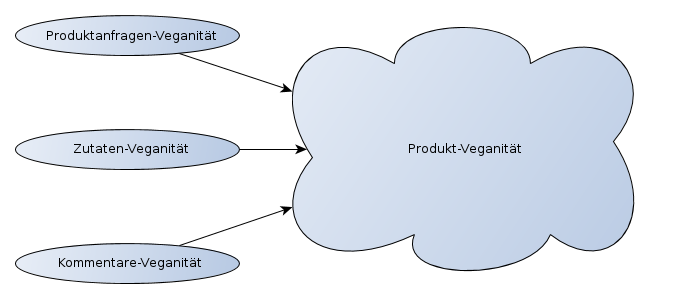
\includegraphics[scale=0.5]{misc/veganity.png}
  \caption{Zusammenhang der einzelnen Veganitäten: Die Veganitäten der Zutaten, 
Produktanfragen und Kommentare berechnen die Produkt-Veganität}
  \label{img:veganity}
\end{figure}

Dafür werden die vier in Abschnitt~\ref{sec:veganity} definierten Veganitäten 
(vegan, unvegan, unklar und unbekannt) verwendet. Ein Produkt ist dabei vegan, 
wenn mindestens eine andere Veganität vegan und keine andere unklar oder 
unvegan ist.\\
Die genaue Berechnung der Produkt-Veganität sowie die der anderen Veganitäten 
wird in Kapitel~\ref{chap:implementation} beschrieben.

\subsection{Erstellung von Zutaten und -informationen}
\label{sec:concept:ingredients}

Zutaten werden entweder bei der Erstellung eines Produktes durch das
Auswerten der Zutatenliste angelegt oder manuell durch das Hinzufügen
einer Zutat.\\
Eine Zutat enthält dabei verschiedene Informationen wie Synonyme,
z.\,B. Beta-Carotin und Carotine bei E160a,
Klassennamen (wie Farbstoff und Säureregulator), ein Bild, eine
Beschreibung, eine Quelle der Beschreibung, Produkte, die diese Zutat
repräsentieren und eine Veganität \citeweb{aid}.\\

\subsection{Generierung von Produktanfragen}
\label{sec:concept:inquiries}

Eine Produktanfrage kann dazu verwendet werden, die Veganität eines
Produktes direkt bei der*dem Hersteller*in durch eine E-Mail zu erfragen.\\
Dies kann bei jedem Produkt erfolgen, allerdings müssen dazu folgende Bedingungen
erfüllt sein:

\begin{itemize}
  \item Die Zutaten-Veganität des Produktes darf nicht unvegan sein, da ansonsten eine Produktanfrage nicht mehr notwendig ist
  \item Ein*e Hersteller*in muss mit zugehöriger E-Mailadresse eingetragen sein
  \item Der*Die Nutzer*in muss eine validierte E-Mailadresse besitzen 
  \item Der*Die Nutzer*in muss die nötigen Befugnisse haben, vgl. 
Abschnitt~\ref{sec:concept:gamification}
\end{itemize}

Die Bedingungen sind dazu da, dass zum einen die Datensätze möglichst
vollständig sind, in diesem Fall der*die Hersteller*in und zum anderen
ein Missbrauch durch die nötigen Befugnisse etwas eingedämmt wird.
Sind diese Bedingungen erfüllt kann eine neue Produktanfrage entweder 
automatisch generiert oder manuell erstellt werden.

Die Anfrage wird dabei als E-Mail an den*die
Hersteller*in
und zugleich noch an den*die Nutzer*in selbst geschickt
sowie zusätzlich unter dem Produkt, zu
dem die Anfrage gestellt wurde, angezeigt.
Der volle Name von der*dem 
Nutzer*in kann dabei anonymisiert werden, wenn dies eingestellt wurde (vgl. 
Abschnitt~\ref{sec:concept:users}).\\
Wird die Produktanfrage beantwortet wird diese Antwort entweder automatisiert
in das System eingefügt oder kann manuell erstellt werden.
Bei der Erstellung besteht die Möglichkeit, eine Veganität festzulegen und die
Produktanfrage "`hervorzuheben"', d.\,h. zu bestätigen, dass das
Produkt nun entweder vegan oder unvegan ist und keine offenen Fragen
mehr vorliegen. Diese Produktanfrage bzw. Antwort auf eine vorherige
Anfrage wird unter einem Produkt auch entsprechend hervorgehoben
angezeigt.

\subsection{Kommentare erstellen}
\label{sec:concept:comments}

Ein Produkt kann von angemeldeten Nutzer*innen kommentiert werden, um
eventuelle Unstimmigkeiten der vorhandenen Angaben aufzuzeigen, eine 
Produktinformation in
Frage zu stellen oder eine Veganität zu spezifizieren.
Zur Spezifizierung können dabei die in Abschnitt~\ref{sec:veganity}
definierten Veganitäten benutzt werden.\\
Die Kommentare werden jeweils mit Datum, Zeit und einem Spitznamen
unterhalb eines Produktes nacheinander
angezeigt und können auch dort erstellt werden.
Wie die Kommentare zur Berechnung der Veganität benutzt werden, ist in
Abschnitt~\ref{sec:implementation:comments} beschrieben.

\subsection{Gamifizierung}
\label{sec:concept:gamification}

Durch die sogenannte "`Gamifizierung"', d.\,h. der Gebrauch von
Elementen aus dem Game-Design in einem anderen Kontext, wird bei den
Nutzer*innen ein Anreiz geschaffen, etwas zu leisten
\cite{chi:gamification-1, chi:gamification-2, sander11}.\\
Dies wird auch in \name benutzt, um
die Datenbank möglichst vollständig zu füllen.\\
Genutzt werden als Elemente der Gamifizierung das Punktesystem (Points system), 
die Fortschrittsanzeige (Progress bar)
und die Bestenliste (Leaderboard) \cite{rta13}.

Punkte können durch die folgenden Aktionen "`verdient"' werden:
\begin{itemize}
  \item Anlegen eines Kommentars
  \item Erstellung eines Produktes
  \item Vollständig ausgefülltes Produkt
  \item Neue Produktanfrage
  \item Validierung der E-Mailadresse
  \item Antwort auf Produktanfrage hinzufügen
\end{itemize}

Diese Aktionen werden unterschiedlich stark "`vergütet"', ein Kommentar z.\,B. 
mit weniger Punkten als ein neues Produkt oder das Einfügen einer Antwort des 
Herstellenden auf eine vorherige Produktanfrage.
Dies soll zu einem Anreiz führen, mehr Produkte bzw. Produktanfragen zu 
erstellen.\\
Allerdings sind einige Aktionen nicht direkt ausführbar, können aber durch 
andere Aktionen bzw. die Punktbelohnung derer freigeschaltet werden:
\begin{itemize}
  \item Kommentar schreiben
  \item Produktanfrage schreiben
  \item Quelle zu Produkt hinzufügen
  \item Zutat manuell erstellen und Zutaten verändern
\end{itemize}

Dies soll einerseits einen Anreiz schaffen, mehr Daten in die Datenbank 
einzugeben um mehr Rechte zu bekommen und andererseits einem Missbrauch 
vorbeugen.
Mehr Rechte wie Einträge löschen und Personen deaktivieren können nur von den 
vorhandenen Administrator*innen vergeben werden.

Eine Bestenliste, welche die Nutzer*innen mit Avatar, Spitzname und
Punktanzahl auflistet, soll für einen kleinen Wettbewerb untereinander
sorgen, wobei dadurch wieder mehr Produkte eingetragen bzw. Einträge
vervollständigt werden sollen.

Eine Fortschrittsanzeige wird unter einem Produkt angezeigt um
zu einem vollständig ausgefüllten Datensatz zu führen und sorgt daher für 
eine Punktbelohnung, sobald alle notwendigen Informationen eingetragen sind.
Einige Informationen wie Merkmale, Siegel, Nährwertangaben, Allergene, Spuren 
und die Quelle werden dabei nicht beachtet, da sie nicht bei jedem Produkt 
vorliegen.

\subsection{Hersteller*in anlegen}
\label{sec:concept:manufacturer}

Direkt bei der Erstellung eines Produktes kann mit der Marke auch
ein*e Hersteller*in angelegt werden.\\
Dabei kann die Information über ein*e Hersteller*in zusätzlich zu
einem Namen noch um ein Logo, eine
Adresse, eine E-Mailadresse, eine Telefon- sowie eine Faxnummer ergänzt werden.
Die E-Mailadresse ist eine Pflichtangabe, sofern eine Produktanfrage
an diese*n Hersteller*in geschickt werden soll, siehe dazu auch
Abschnitt~\ref{sec:inquiry}.
Zusätzlich zu den genannten Angaben werden auf der Übersichtsseite des 
Herstellenden die Marken aufgelistet, die
zu diesem*dieser Hersteller*in gehören.